\section{Library \mylib{vignette}}\label{sec:vignette}%
\tcbset{external/prefix=external/vignette_}%
The library is loaded by a package option or inside the preamble by:

该库可以通过包选项或在导言区中加载:
\begin{dispListing}
\tcbuselibrary{vignette}
\end{dispListing}
This also loads the \mylib{skins} library, see \Fullref{sec:skins},
and the |fadings| library of |tikz| .

这也加载了\mylib{skins}库,请参见\Fullref{sec:skins},以及|tikz|的|fadings|库。
\subsection{Vignette Drawing\\镜框绘制}\label{subsec:vignettedrawing}

\begin{docCommand}[doc new=2016-04-22]{tcbvignette}{\marg{options}}
In this context, a \emph{vignette} is a four part rectangular frame.
It is constructed as several \tikzname\ paths and, therefore, can only be
used inside a |tikzpicture| environment or inside \refEnvLe{tcolorbox} options.

在这个环境下,\emph{镜框}是一个由四个部分构成的矩形框架。它由多个\tikzname 路径构成,因此只能在|tikzpicture|环境或\refEnvLe{tcolorbox}选项中使用。

The \meta{options} control position, size and style settings of the vignette.
Theses options have the common key path |/tcb/vig/| and are described in
the following.

\meta{选项}控制着镶边的位置、大小和样式设置。这些选项具有共同的关键路径 |/tcb/vig/|,并在下面进行描述。

The next examples show direct \refComLe{tcbvignette} usage without
a \refEnvLe{tcolorbox}.

下面的示例展示了如何直接使用\refComLe{tcbvignette},而不需要\refEnvLe{tcolorbox}。
\begin{dispExample*}{sbs,righthand width=3cm,center lower}
\begin{tikzpicture}
  \tcbvignette{}
\end{tikzpicture}
\end{dispExample*}

\begin{dispExample*}{sbs,righthand width=3cm,center lower}
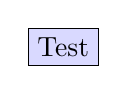
\begin{tikzpicture}
  \node[draw,fill=blue!15!white] (A) {Test};
  \tcbvignette{outside node=A,raised color=blue}
\end{tikzpicture}
\end{dispExample*}

\begin{dispExample*}{sbs,righthand width=3cm,center lower}
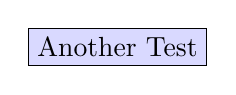
\begin{tikzpicture}
  \node[draw,fill=blue!15!white] (A) {Another Test};
  \tcbvignette{size=3mm,outside node=A,
    north style=red,east style=yellow,
    south style=blue,west style=green}
\end{tikzpicture}
\end{dispExample*}

\begin{dispExample*}{sbs,righthand width=3cm,center lower}

\begin{tikzpicture}
  \node[inner sep=3mm,fill=red!75] (A) {Test};
  \tcbvignette{over node=A,fade in}
\end{tikzpicture}
\end{dispExample*}

\refComLe{tcbvignette} can be used directly inside appropriate options keys
for \refEnvLe{tcolorbox}. Note that options like \refKeyLe{/tcb/underlay} need
\refKeyLe{/tcb/enhanced} or similar settings.

\refComLe{tcbvignette}可以直接在\refEnvLe{tcolorbox}的适当选项键内使用。请注意,像\refKeyLe{/tcb/underlay}这样的选项需要\refKeyLe{/tcb/enhanced}或类似的设置。

\begin{dispExample*}{sbs,righthand width=3cm,center lower}
\begin{tcolorbox}[enhanced,size=small,sharp corners,
  colback=green!10,colframe=green!50!black,
  boxrule=1mm,titlerule=0mm,
  title=My title,center title,fonttitle=\bfseries,
  underlay={\tcbvignette{size=1mm,inside node=frame,
      raised color=green!50!black}}]
    This is a tcolorbox.
\end{tcolorbox}
\end{dispExample*}

Mostly, convenient short cuts like \refKeyLe{/tcb/underlay vignette} can
be used to add a \emph{vignette} to a \refEnvLe{tcolorbox}. Here, \refComLe{tcbvignette}
is used internally.

通常,可以使用方便的快捷方式,如\refKeyLe{/tcb/underlay vignette},向\refEnvLe{tcolorbox}添加一个\emph{vignette}。这里,内部使用了\refComLe{tcbvignette}。

\begin{dispExample*}{sbs,righthand width=3cm,center lower}
\begin{tcolorbox}[enhanced,size=small,sharp corners,
  colback=green!10,colframe=green!50!black,
  boxrule=1mm,titlerule=0mm,
  title=My title,center title,fonttitle=\bfseries,
  underlay vignette]
    This is a tcolorbox.
\end{tcolorbox}
\end{dispExample*}

\end{docCommand}